\chapter{Some Mathematical Preliminaries}
\section{Calculus of Variations}
\label{sec:calc_var}

The calculus of variations is the main tool used in understanding variational forms of mechanics. The basic idea of the calculus of variations is to take the familiar concept of minimizing functions $f(x)$ defined on the real number line $\reals$ and extend it. In your first calculus course, you learned that if $x_0$ was a minimum of $f(x)$, then $\eval{\qty(\dv{f}{x})}_{x_0} = 0$. \marginnote{$\eval{\qty(\dv{f}{x})}_{x_0}$ means ``take the derivative of $f(x)$ with respect to $x$, then set $x = x_0$''. The line means to \emph{evaluate} what comes before it. But do it after taking the derivative, not before!!}
The calculus of variations extends this idea to \textbf{functionals}. A functional takes as \emph{input} a function $f(x)$ and \emph{outputs} a real number, much in the same way an ordinary function takes a real (or complex) number and outputs another real (or complex) number.

The basic idea is just to take a functional and see that something corresponding to its ``derivative'' is zero for the function $f_0(x)$ that minimizes or maximizes the functional. We have to be careful about what that exactly means; it's not the same thing as the derivative of a function. However, it turns out that once we figure out what we're doing, the calculus of variations will use only the standard techniques of calculus you already know. Doing this will give you extremely useful insights into the function $f_0(x)$ that minimizes the functional. 

\marginnote{Functionals are typically written like this $J[y]$, where $y(x)$ is a function. Note the square brackets rather than parantheses. Don't mix them up!}

\subsection{A simple example}
Imagine you a have a function $y(x)$ that defines a curve in the $x-y$ plane. A functional you might care about is the \emph{length} of the curve. We are going to demonstrate that the shortest path between two points in a Cartesian plane is a straight line. While this is likely not news to you, it is a simple example that demonstrates what the calculus of variations does.

First, let's consider a simple curve in the plane defined by $y(x)$. What is its length? Formally, length is the sum of the lengths of straight lines with their endpoints on the curve as the length of those straight lines goes to zero. 
\begin{marginfigure}
  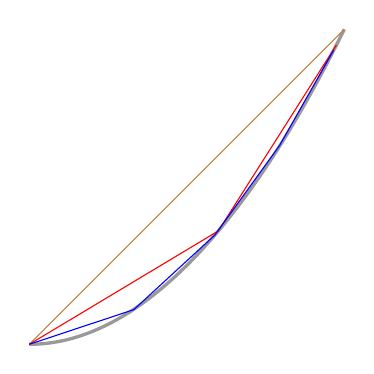
\begin{tikzpicture}
    \draw[very thick, opacity=0.4] (0,0) parabola (4,4);
    % one segment
    \draw[brown] (0,0) -- (4,4);
    % two segments
    \draw[red] (0.000000, 0.000000) -- (2.39903577440834945689, 1.43884316172276724673);
    \draw[red] (2.39903577440834945689, 1.43884316172276724673) -- (3.89884347400339059675, 3.80024510869470687200);
    % four segments
    \draw[blue] (0.000000, 0.000000) -- (1.32751778757082461161, 0.440575869079234254915);
    \draw[blue] (1.32751778757082461161, 0.440575869079234254915) -- (2.35637792872391482746, 1.38812923574430175672);
    \draw[blue] (2.35637792872391482746, 1.38812923574430175672) -- (3.17591368982622146433, 2.52160694130640120978);
    \draw[blue] (3.17591368982622146433, 2.52160694130640120978) -- (3.86669943908696955859, 3.73784113805887125195);    
  \end{tikzpicture}
  \caption{The sum of the lengths of these line segments limits to the length of the curve.}
\end{marginfigure}
Given that definition and the length of a straight line,
\begin{equation}
  \label{eq:line_seg}
  s = \sqrt{(x_1 - x_0)^2 + (y_1 - y_0)^2},  
\end{equation}
the length of the curve is given by
\begin{equation}
  \label{eq:curve_length_1}
  L[y] = \int_a^b ds.
\end{equation}
This is our first functional. We can put this in terms of $dx$ to arrive at the more useful form
\begin{equation}
  \label{eq:curve_length_final}
  L[y] = \int_a^b \sqrt{1 + y'(x)} dx.
\end{equation}

\begin{Exercise}
  Derive equation~(\ref{eq:curve_length_final}). Use equation~(\ref{eq:line_seg}).
\end{Exercise}

Now that we have a functional for the length of a curve $y(x)$, we will show that a straight line, $y_0 = mx$, is in fact the shortest path between any two points. For simplicity, we'll take $a = 0$ and $b = 1$. In order to show this, we will demonstrate that any function $y(x) = y_0(x) + \epsilon \delta y(x)$ is longer than $y_0(x)$.\marginnote{Let's be careful about notation here. $\delta y(x)$ is a \emph{function} of $x$, just like $y(x)$. $\epsilon$ is a constant; almost always when you see $\epsilon$, you should assume it's a \emph{small} constant. Unfortunately, traditional notation is a bit confusing. The $\delta$ in $\delta y$ is just a part of the \emph{name} of the function. It's not an operator like $\dv{x}$.} The first thing we need to know about $\delta y(x)$ is that $\delta(b) = \delta(a) = 0$. If this weren't true, then the new function $y_0(x) + \epsilon \delta y(x)$ would not satisfy the boundary conditions for arbitrary $\epsilon$ because $y_0(x)$ \emph{does}.

Let's look at the length functional for $y + \epsilon \delta y$:
\begin{equation}
  \label{eq:line_perturb_length}
  L[y_0 + \epsilon \delta y] = \int_0^1 \sqrt{1 + (y_0' + \epsilon \delta y')^2 } dx.
\end{equation}
Now $L[y_0 + \epsilon \delta y]$ is a \emph{functional} of $y_0 + \epsilon \delta y$, but it's a \emph{function} of $\epsilon$. So, if we want to find the minimum, we can simply take the derivative with respect to $\epsilon$ and evaluate at $\epsilon = 0$,
\begin{equation}
  \begin{split}
    \label{eq:deriv_length}
    \eval{\dv{L[y_0 + \epsilon \delta y]}{\epsilon}}_{\epsilon=0} & = \int_0^1 \sqrt{1 + (m + \epsilon \delta y')^2 } dx.\\
    & = \frac{m}{\sqrt{1 + m^2}} \qty(\delta y(1) - \delta y(0))\\
    & = 0.\\
  \end{split}
\end{equation}
This tells us that $\epsilon = 0$ is an \emph{extrema}. To find out if it's a minimum or a maximum, we need to use its second derivative.
\begin{Exercise}
  Show that $\eval{\dv[2]{L[y_0 + \epsilon \delta y]}{\epsilon}}_{\epsilon = 0} > 0$ and thus $\epsilon = 0$ is a minimum.
\end{Exercise}

Thus, we see that $y_0 = mx$ is indeed the shortest path. But there's a weakness to this: we had to know what $y_0(x)$ was. It turns out that the calculus of variations is so useful because we can use it to find extremal paths without knowing what they are.

\subsection{Functional Variations}
We want to find the minima of a functional, and we can show that we can do that using only standard calculus techniques. In essense, we are going to turn the problem of minimizing a functional into an ordinary differential equation in $x$.

Let's start by defining the functional $J[y]$,
\begin{equation}
  \label{eq:generic_functional}
  J[y] = \int_a^b F(x, y, y') dx,
\end{equation}
in terms of a \emph{function} $F(x, y, z)$ that has continuous first and second derivatives in all of its three arguments. We want to find stationary points\marginnote{A ``stationary'' point is an extrema, a minimum or maximum. Luckily for us, we're usually only interested whether or not a given function yields a stationary point of the functional, not whether it is a minimum or maximum.}  of this functional by turning it into a set of ordinary differential equations.

To do so, let's introduce the \textbf{first order functional variation}
\begin{equation}
  \label{eq:first_order_functional_variation}
  \begin{split}
    \var{J[y]} & \equiv \eval{\qty(\dv{J[y_0+\epsilon \delta y]}{\epsilon})}_{\epsilon=0}\\
    & = \int_a^b \qty[\dv{F(x, y_0 + \epsilon \delta y, y_0' + \epsilon \delta y')}{\epsilon}]_{\epsilon = 0} dx,    
  \end{split}
\end{equation}
where here we note that in the expression $\var{J[y]}$, $\delta$ is an \textbf{operator}, but in $\delta y(x)$, it's just the name of the function. Now, we make use of the chain rule\marginnote{The chain rule is something you should know cold. It's $\dv{f(g(x))}{x} = \dv{f}{g} \dv{g}{x}$} as applied to a multivarible function , $F(x, y(x), y'(x))$:

\begin{equation}
  \label{eq:chain_rule}
  \dv{F}{\epsilon} = \pdv{F}{x} \dv{x}{\epsilon} + \pdv{F}{y} \dv{y}{\epsilon} + \pdv{F}{y'} \dv{y'}{\epsilon}.
\end{equation}
The first term is zero because $x$ is independent of $\epsilon$. Substituting $y_0 + \epsilon \delta y$ for $y$ and similarly for $\delta y$, we end up with
\begin{equation}
  \label{eq:first_order_functional_step2}
    \var{J[y]} = \int_a^b \qty[\pdv{F}{y} \delta y + \pdv{F}{y'} \delta y']_{\epsilon = 0} dx.
\end{equation}
We want to integrate the second term by parts because it's in the canonical form, and because 

\subsection{References}
\begin{itemize}
\item Princeton Companion, III.94 ``Variational Methods'', Lawrence C. Evans
\item Brizard, ``An Introduction to Lagrangian Mechanics''
\end{itemize}

% \subsection{Sets and Spaces}
% \label{sec:sets_spaces}

% If you want to read some more mathematical references, it's very handy to know the very basics of set-builder notation. See the appendix. 


% \appendix

% \section{Set-Builder notation}
% \label{sec:set-builder}

% A \emph{set} is written between curly braces: \{3, 4, 7, 2\} is the set of digits that make up the first six digits of my telephone number. More often, we're intersted in sets that can't be written out explicitly. Some sets are so well known, we don't even need to do more than use their names. For example,
% \begin{itemize}
% \item \mathbb{R}: the set of all real numbers
% \item \mathbb{Z}: the set of integers (for the interested, \emph{zahlen} is German for ``integer'')
% \item \mathbb{C}: the set of all complex numbers
% \end{itemize}
% are three sets you'll run into in physics.

% For most other sets of interest, we use ``set builder'' notation, which gives a set of things with conditions for membership. There are always three parts: a \emph{variable}, either | or :, and then a condition (properly called a \emph{predicate}). So